\documentclass{scrreprt}
\usepackage{listings}
\usepackage{underscore}
\usepackage{graphicx}
\usepackage[bookmarks=true]{hyperref}
\usepackage[utf8]{inputenc}
\usepackage[english]{babel}
\hypersetup{
    bookmarks=false,    % show bookmarks bar?
    pdftitle={Software Requirement Specification},    % title
    pdfauthor={Jean-Philippe Eisenbarth},                     % author
    pdfsubject={TeX and LaTeX},                        % subject of the document
    pdfkeywords={TeX, LaTeX, graphics, images}, % list of keywords
    colorlinks=true,       % false: boxed links; true: colored links
    linkcolor=blue,       % color of internal links
    citecolor=black,       % color of links to bibliography
    filecolor=black,        % color of file links
    urlcolor=blue,        % color of external links
    linktoc=page            % only page is linked
}%
\def\myversion{1.0 }
\date{}
%\title
\usepackage{hyperref}
\begin{document}

\begin{flushright}
    \rule{16cm}{5pt}\vskip1cm
    \begin{bfseries}
        \Huge{USER MANUAL}\\
        \vspace{1.5cm}
        for\\
        \vspace{1.5cm}
        CULater\\
        \vspace{1.5cm}
        \LARGE{Version \myversion}\\
        \vspace{1.5cm}
        Prepared by : Group A1\\
        \vspace{1.5cm}
        Submitted to : Prof. Tak-Kei Lam\\CSCI3100 Instructor\\
        \vspace{1.5cm}
        \today\\
    \end{bfseries}
\end{flushright}

\newpage
\tableofcontents
\newpage
\chapter{Introduction}

CULater is a Web based planner application designed specifically for the Chinese University of Hong Kong (CUHK) community, facilitating the creation and management of tasks for individual users, as well as for student groups, university departments, and other school related groups/organizations. It addresses the need for a centralized platform where CUHK members can efficiently manage their academic and extracurricular commitments.\\

The primary objective of this product is to simplify the organization of academic and social activities, solve the problem of fragmented communication and scheduling by providing a cohesive tool that keeps everyone informed and organized, hence improving collaboration between students and faculty. By allowing users to create and manage groups, and share group related tasks, CULater hopes to encourage a more connected and active campus environment. \\

This document is a user manual explaining the functionalities of CULater. Step-by-step instructions are given to perform specific actions such as signing up, logging in, creating groups, leaving groups, etc. Additionally, relevant information about processes will be specified.

\chapter{Signing Up}

When you first open the application, you will be on the login page. If you already have an account, preceed with logging in (see Chapter 3: Login). If you don't have an account, proceed to the signup page by clicking on the "Sign Up" box below the "LOGIN" box. See Figure 2.1.\\
\begin{figure}[htbp]
        \centering
        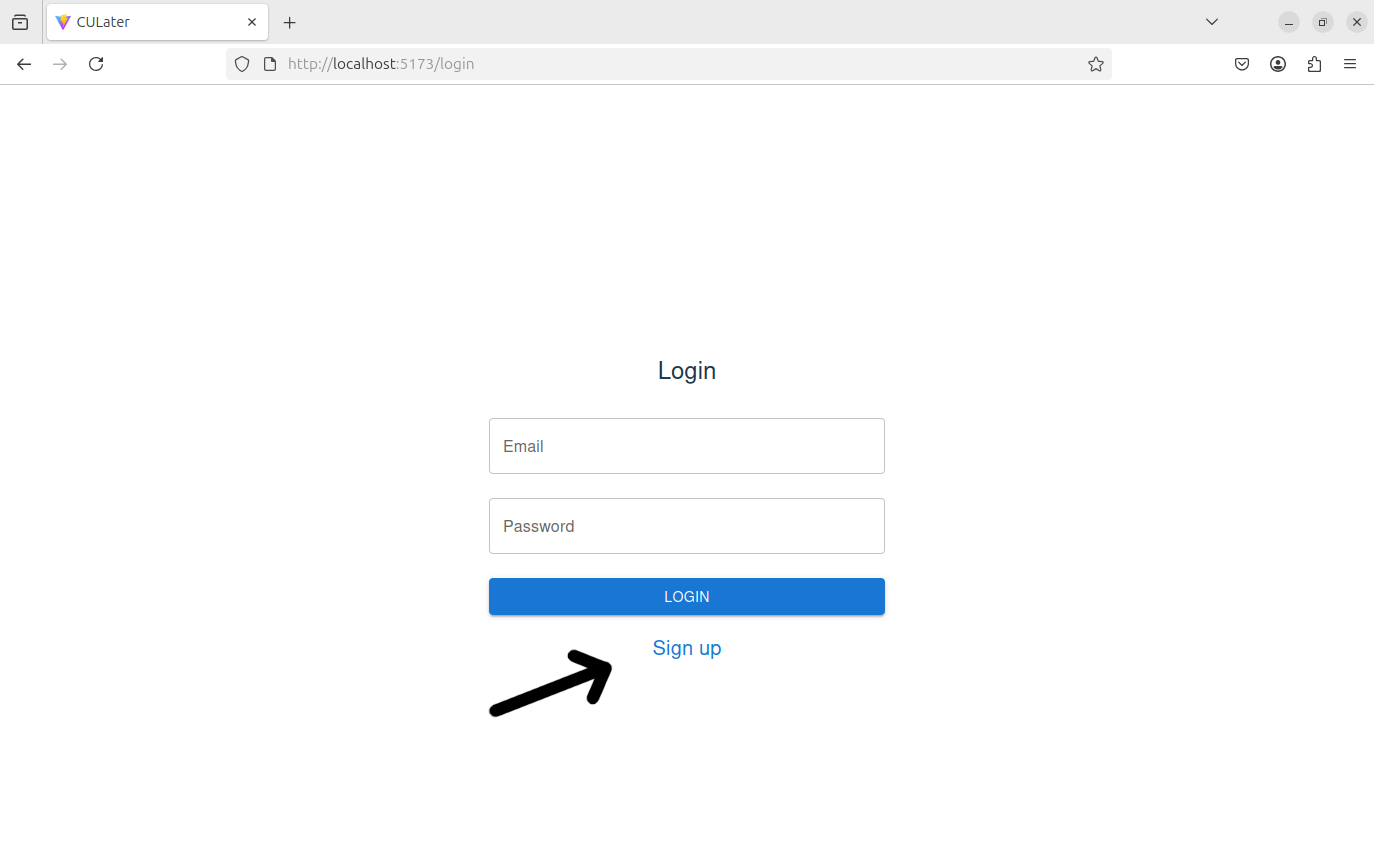
\includegraphics[width=0.8\textwidth]{login_page_arrow_signup.png}
	\caption{Login page}
	\label{fig:my_label}
\end{figure}

To create an account, enter a valid email address in the "Email" field, a valid password in the "Password" field, and a valid software license key in the "License Key" field. A valid email address can be used to create only a single account. If another account is attempted to be created using an email address that is already linked to another account, an error message will be prompted. The password must be between 8-32 characters and contain at least one uppercase letter, one lowercase letter, one numbers, and one special character. If an invalid password has been entered, an error will be prompted. The software license key is a one-time license key used to create your account. These keys are obtained directly by contacting the product team at \href{mailto:culater@support.hk}{culater@support.hk}. A license key can be used to create a single account. Once it's used to create an account, it cannot be used to create another account. If a used license key is entered in an attempt to create a new account, an error message will be prompted. See Figure 2.2.\\
\begin{figure}[htbp]
        \centering
        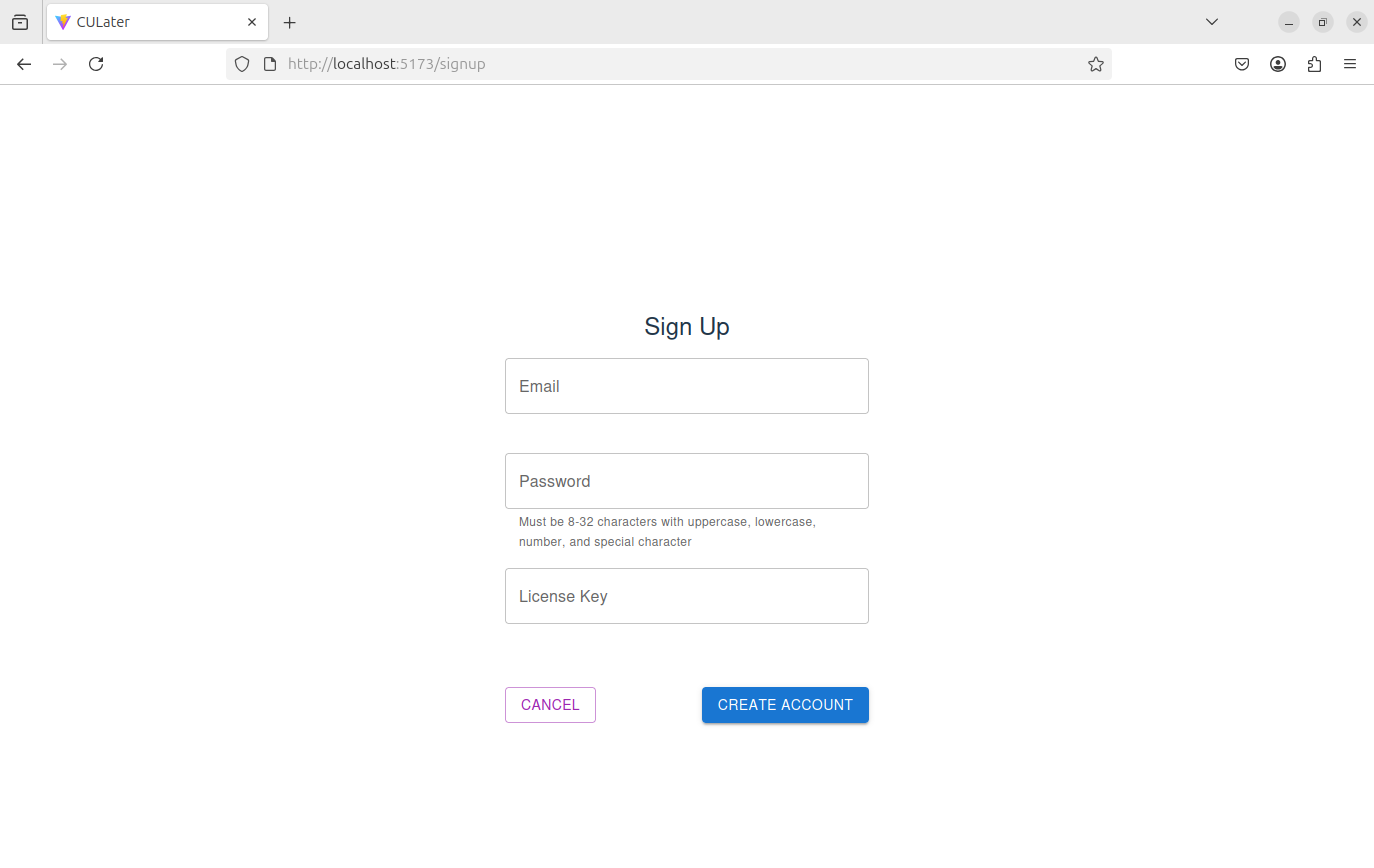
\includegraphics[width=0.8\textwidth]{sign_up_page.png}
	\caption{Sign up page}
	\label{fig:my_label}
\end{figure}

\chapter{Login}

Once you successfully created an account, the application will automatically take you to the login page. Enter your email address and your password, then click on the "LOGIN" box. If your credentials are incorrect, an error will be prompted. See Figure 3.1.\\
\begin{figure}[htbp]
        \centering
        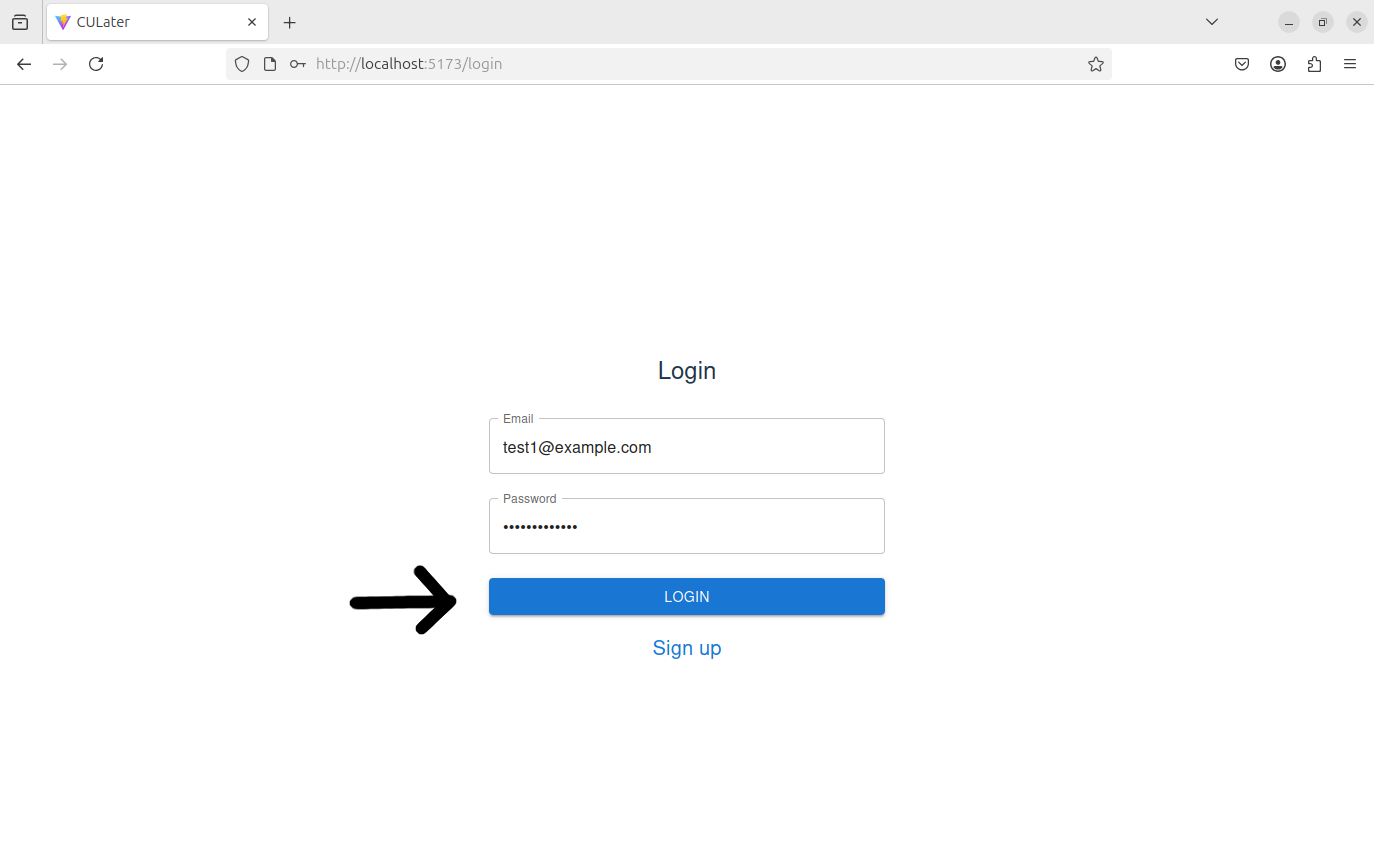
\includegraphics[width=0.8\textwidth]{login_credentials_entered_w_arrow.png}
	\caption{Login page}
	\label{fig:my_label}
\end{figure}

\chapter{Logout}

Once you are logged in, if you want to logout, click on the "LOGOUT" box on the top right corner of your dashboard. This will securely log you out. Next time you open the application, you will need to login again. If you close the application without logging out, you will stay logged in. So the next time you open the application again, you will directly see your dashboard. See Figure 4.1.\\
\begin{figure}[htbp]
        \centering
        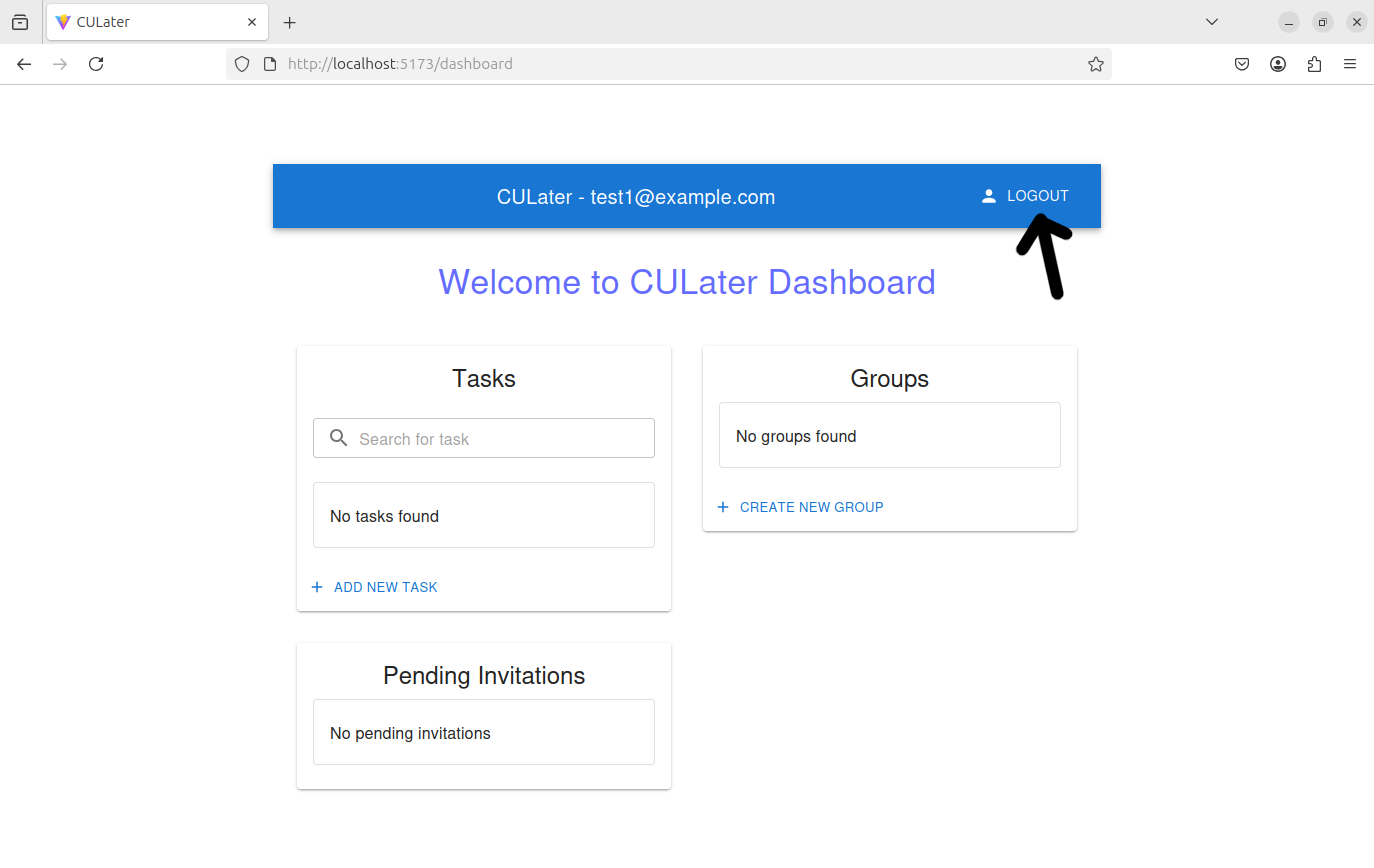
\includegraphics[width=0.8\textwidth]{logout.png}
	\caption{Logout}
	\label{fig:my_label}
\end{figure}

\chapter{Group Creation}

To use CULater, you will have to create or be a member of groups. Without groups, you cannot create tasks. If you would like to create a new group, click on "+ CREATE A NEW GROUP" on your dashboard under the "Groups" tab. Once you click this box, you will be prompted with a group creation page. Here, there are two fields to fill out: the group name and a description. To create a group, you must fill out the "Group Name" field. The "Description" field is optional. Once you filled out the fields, click "OK". Click "CANCEL" if you would like to cancel the group creation. Once you have successfully created a new group, it will be displayed on your dashboard. See Figure 5.1-5.3.\\
\begin{figure}[htbp]
        \centering
        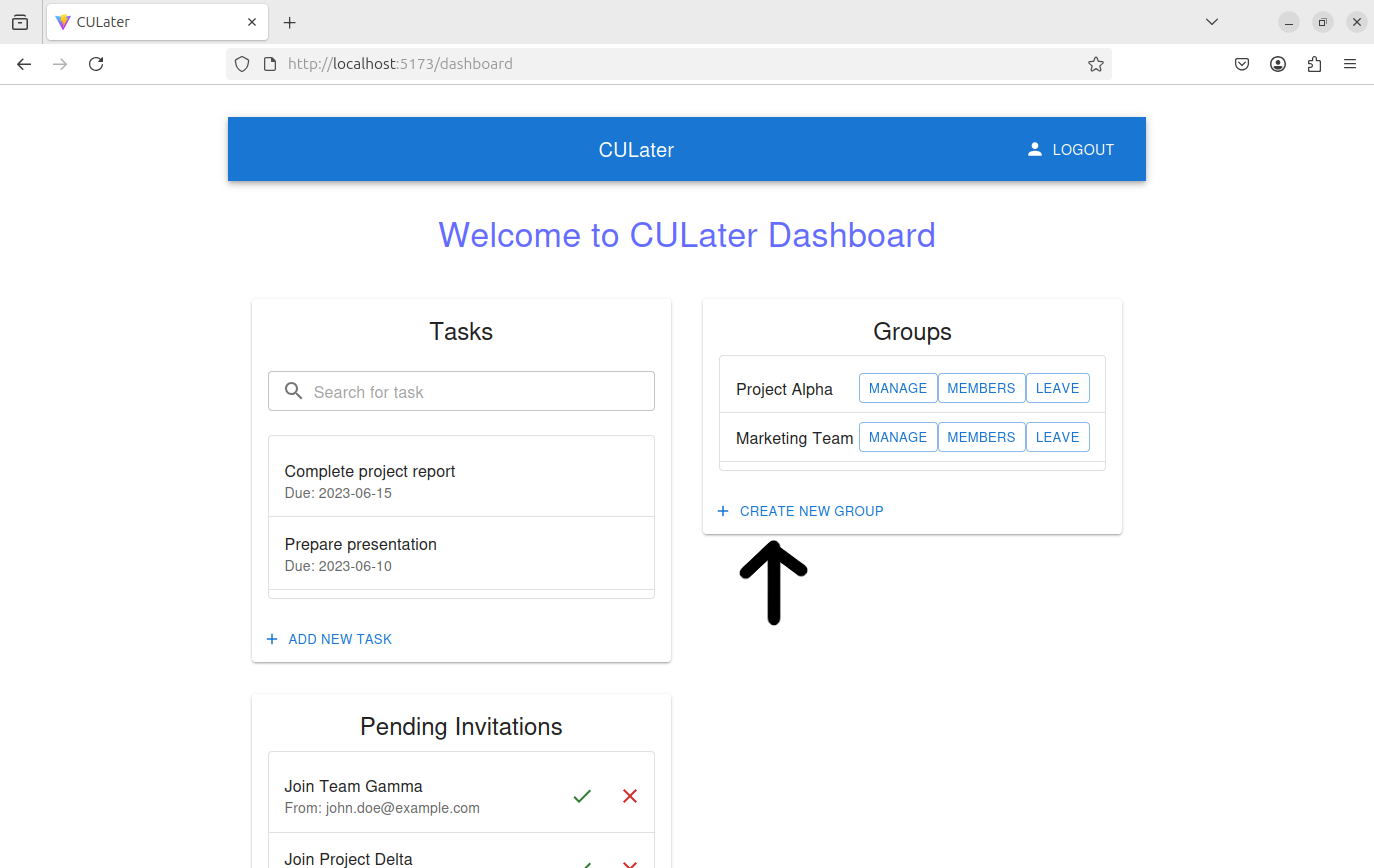
\includegraphics[width=0.8\textwidth]{dahboard_with_tasks_and_groups_and_invites_create_group.png}
	\caption{Create a new group}
	\label{fig:my_label}
\end{figure}
\begin{figure}[htbp]
        \centering
        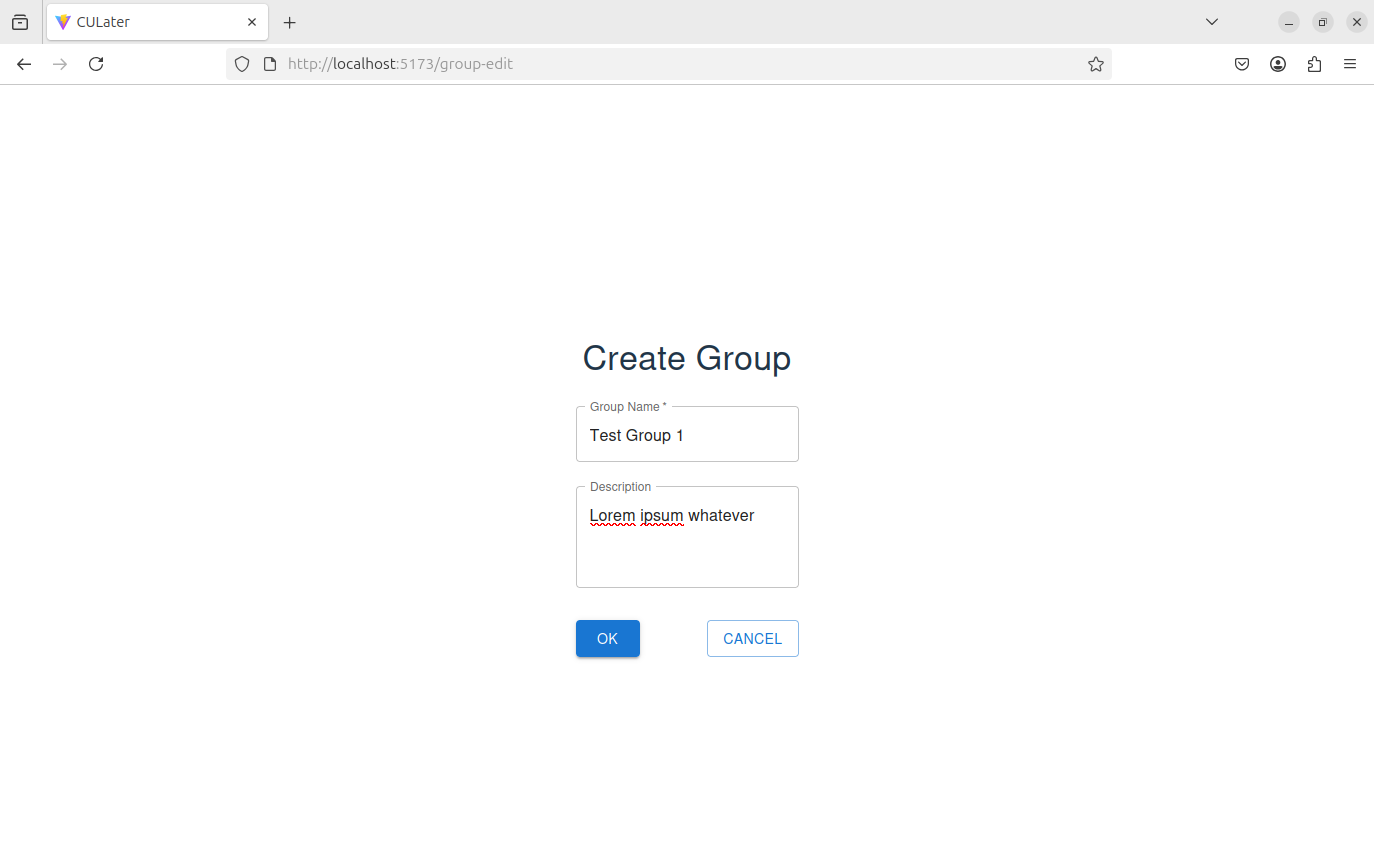
\includegraphics[width=0.8\textwidth]{group_creation.png}
	\caption{Group creation page}
	\label{fig:my_label}
\end{figure}
\begin{figure}[htbp]
        \centering
        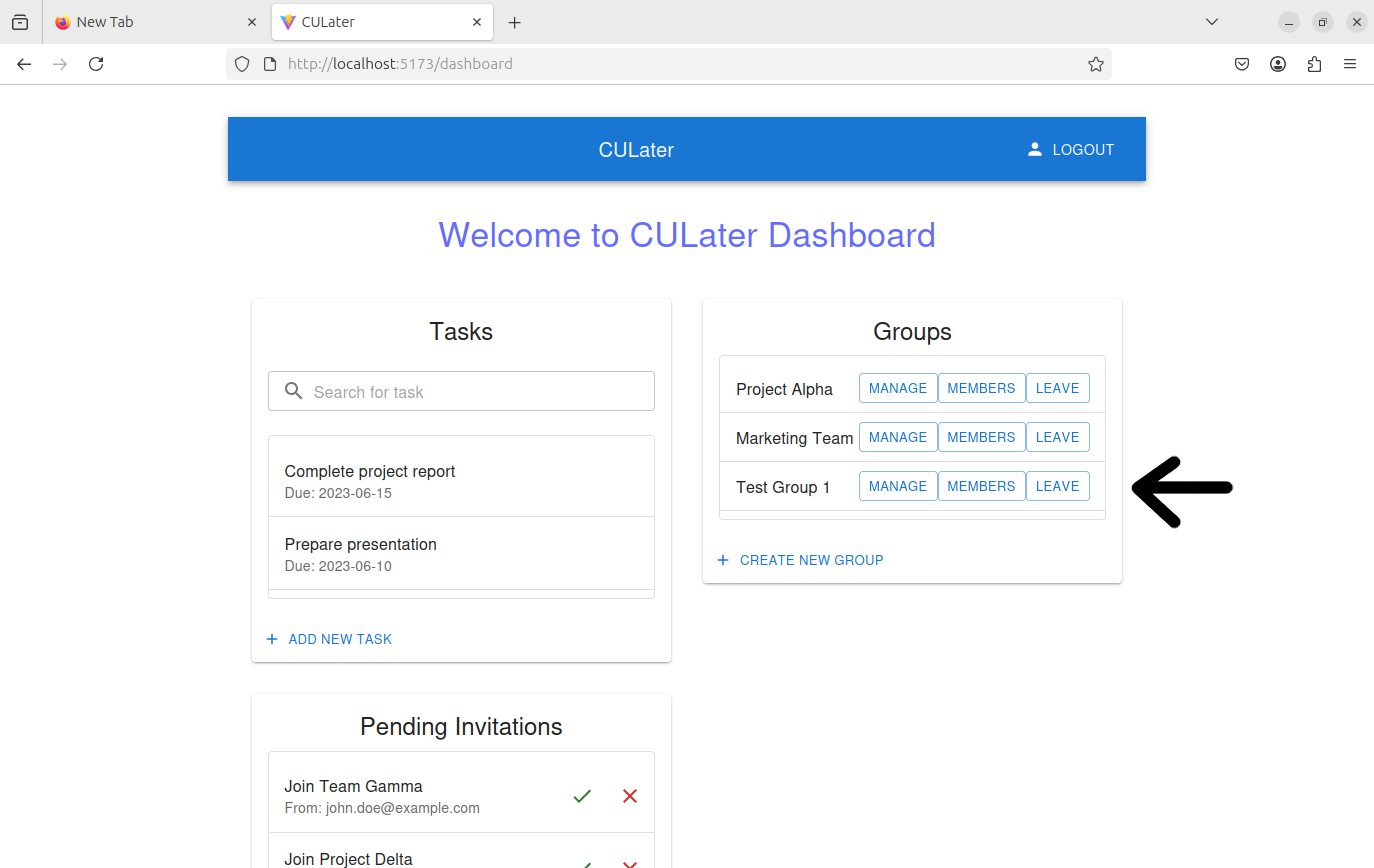
\includegraphics[width=0.8\textwidth]{added_new_group_dashboard.png}
	\caption{Dashboard with the new group}
	\label{fig:my_label}
\end{figure}

\chapter{Group Roles}
In a group, there are three kinds of users. A user must have one, and only one, of these three roles:

\begin{itemize}
	\item Admins
	\item Contributors
	\item Readers
\end{itemize}

Each role comens with its own scope of actions. Readers can only view the details and tasks of a group. Contributors can do everything readers can do, along with inviting other users to the group as Readers, and creating tasks in the group. Admins can do everything Contributors can do, along with updating the group details.

\chapter{Task Creation}

For task creation, you need to have groups. Each task you create needs to belong to a group. To create a task, click on "+ ADD NEW TASK" on your dashboard. If you currently do not have any groups, you will be prompted with an error. Click "OK" once you get the error, and you will be prompted with a group creation window. Enter the name of the group you would like to create, and click "OK". Once you click "OK", a new group will be created, and you can proceed with the task creation process. If you click "CANCEL" a new group won't be created, and you won't be able to add a new task.\\

Once there are groups where you are either an admin or a contributor, you can create tasks. When you click "+ ADD NEW TASK" on your dashboard, you are prompted with the required fields to create the task. Fields with "*" mean they are mandatory. The only mandatory field is the title of the task. Description and due date fields are optional. Then, you must choose one group to assign the task to. Once you submit, the task is created, and it will appear on your dashboard.\\

\textbf{Note:} To be able to create tasks in a group, you have to be an admin or a contributor in that group. Refer to Chapter 6: Group Roles.\\
\begin{figure}[htbp]
        \centering
        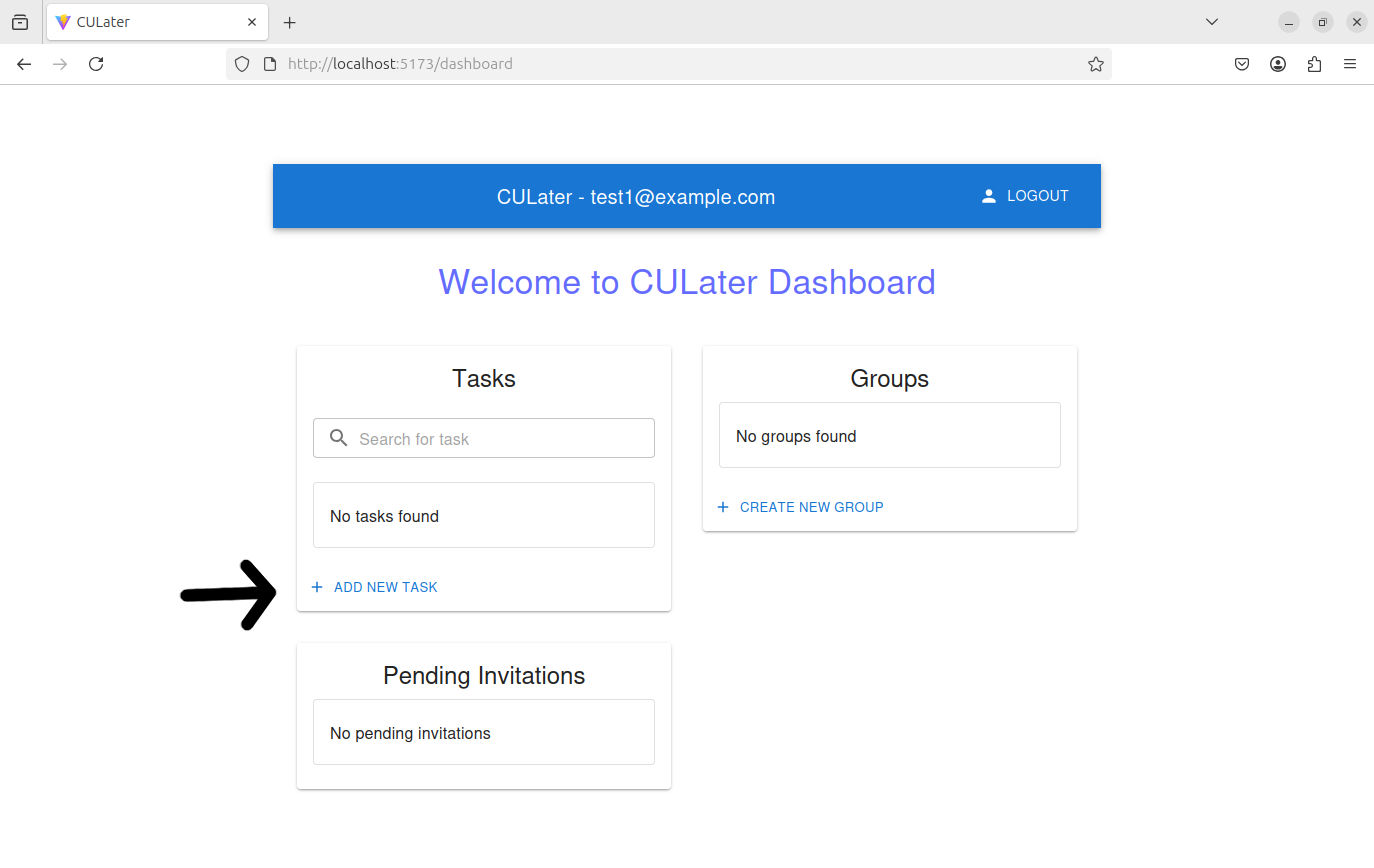
\includegraphics[width=0.8\textwidth]{dashboard_add_task.png}
	\caption{Adding a new task}
	\label{fig:my_label}
\end{figure}
\begin{figure}[htbp]
        \centering
        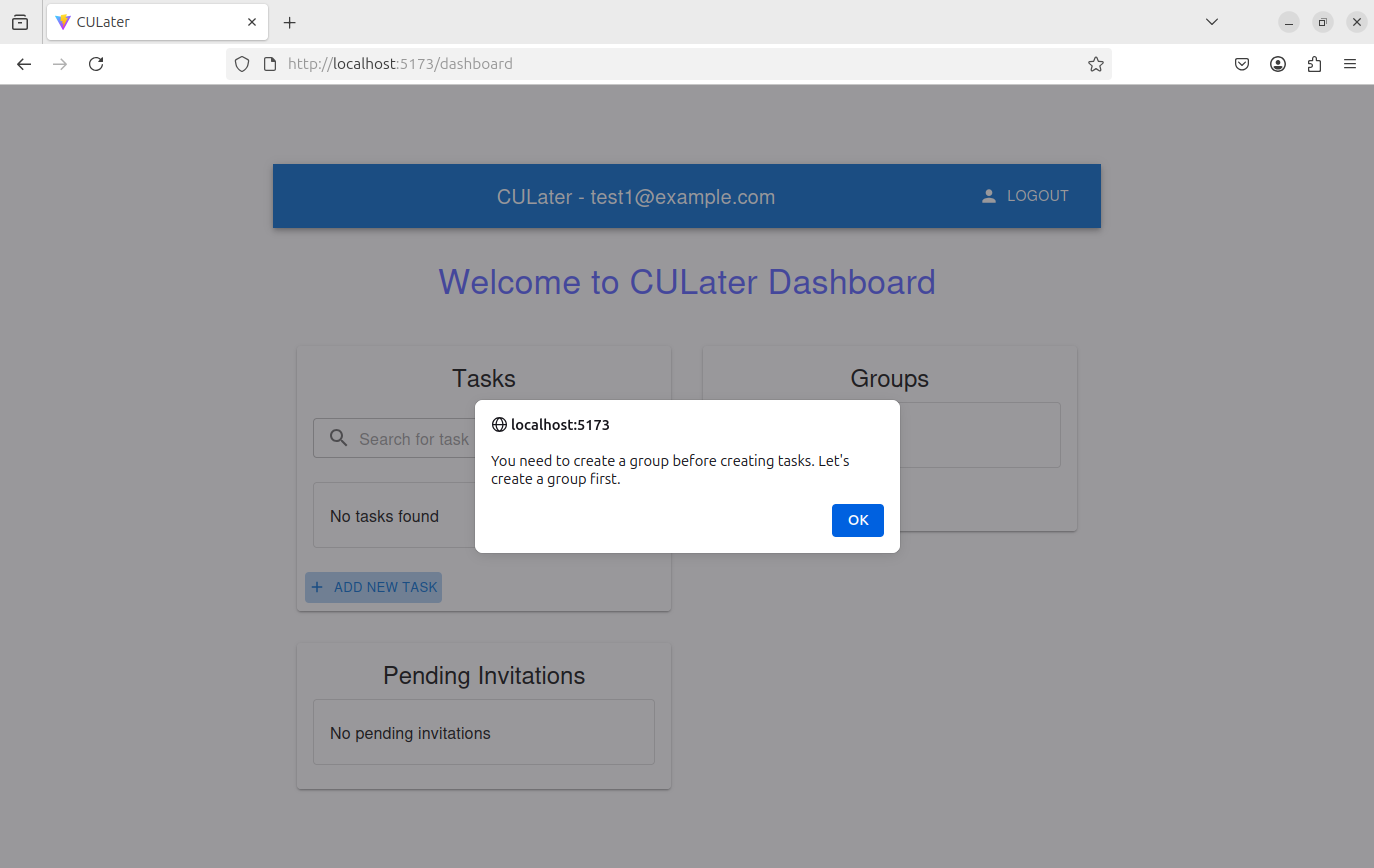
\includegraphics[width=0.8\textwidth]{create_task_no_group.png}
	\caption{No groups error}
	\label{fig:my_label}
\end{figure}
\begin{figure}[htbp]
        \centering
        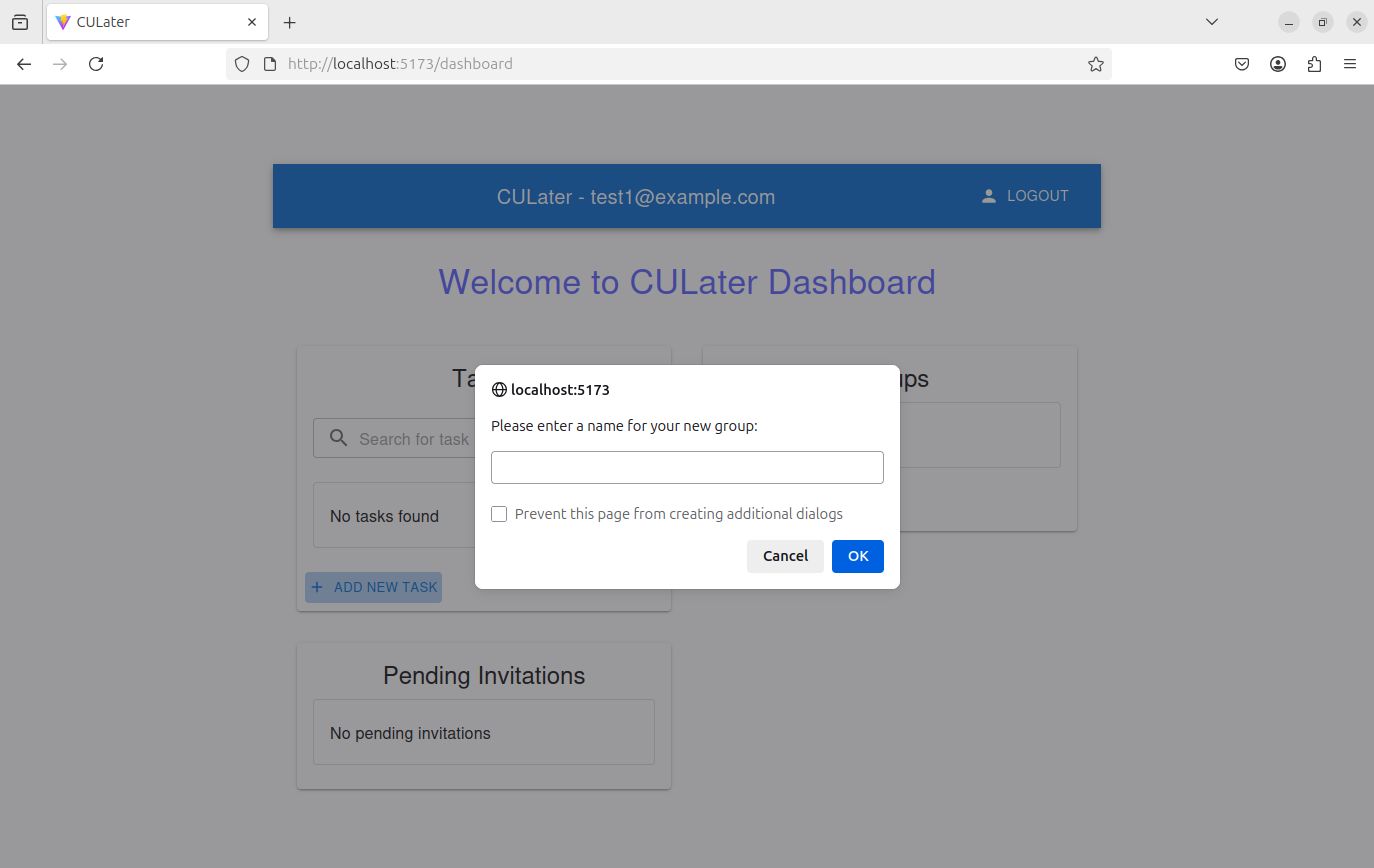
\includegraphics[width=0.8\textwidth]{task_create_no_group_new_group_creation.png}
	\caption{New group creation}
	\label{fig:my_label}
\end{figure}

% UNCOMMENT ONCE BUGS ARE FIXED, TASK CREATION PAGE
%\begin{figure}[htbp]
        %\centering
        %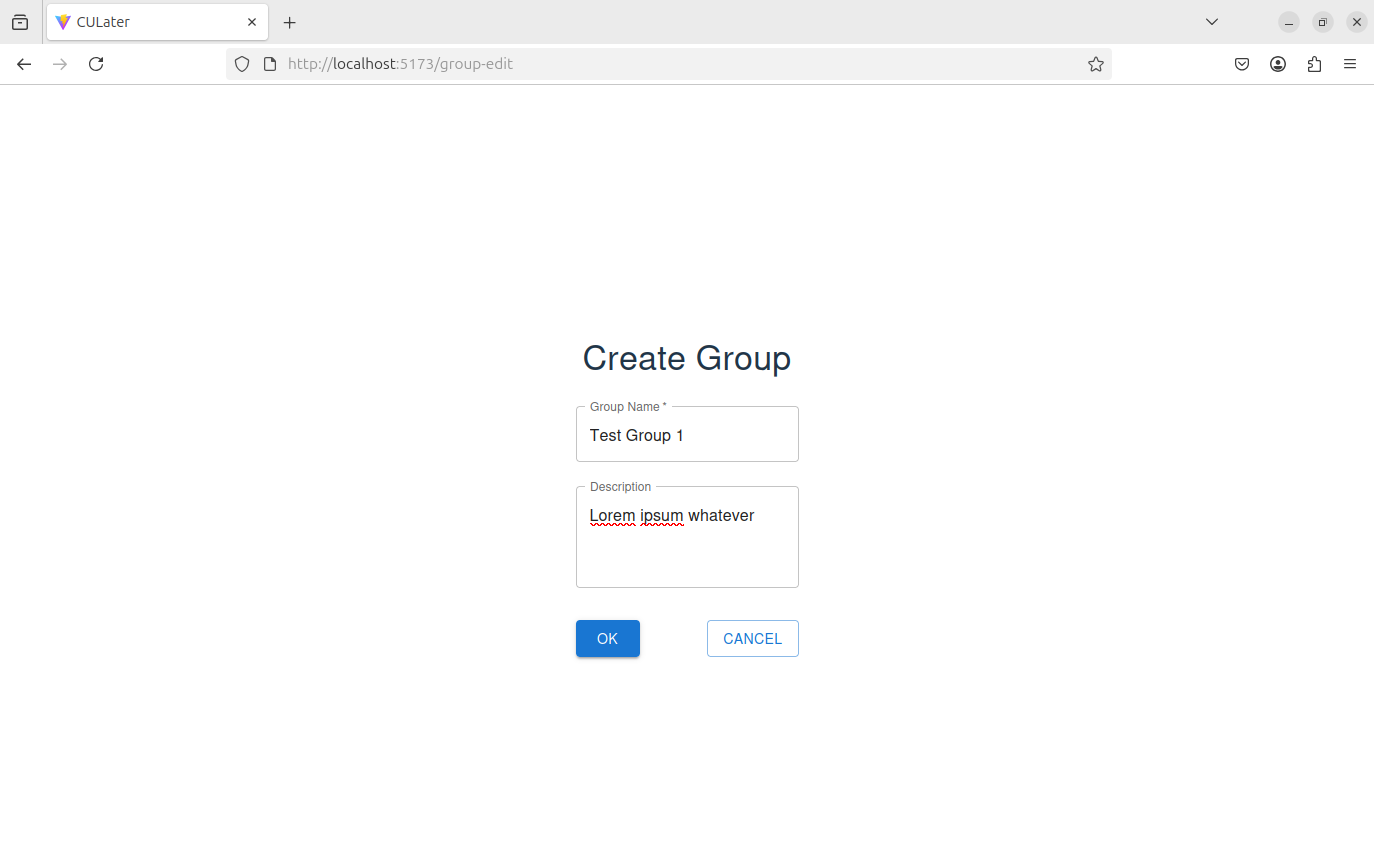
\includegraphics[width=0.8\textwidth]{group_creation.png}
	%\caption{Task creation}
	%\label{fig:my_label}
%\end{figure}

\chapter{Task Filtering}

At the top of the "Tasks" tab on the dashboard, there is a search bar. You can type the group name of the tasks you would like to view, and only the tasks belonging to the specified group will be shown.
\begin{figure}[htbp]
        \centering
        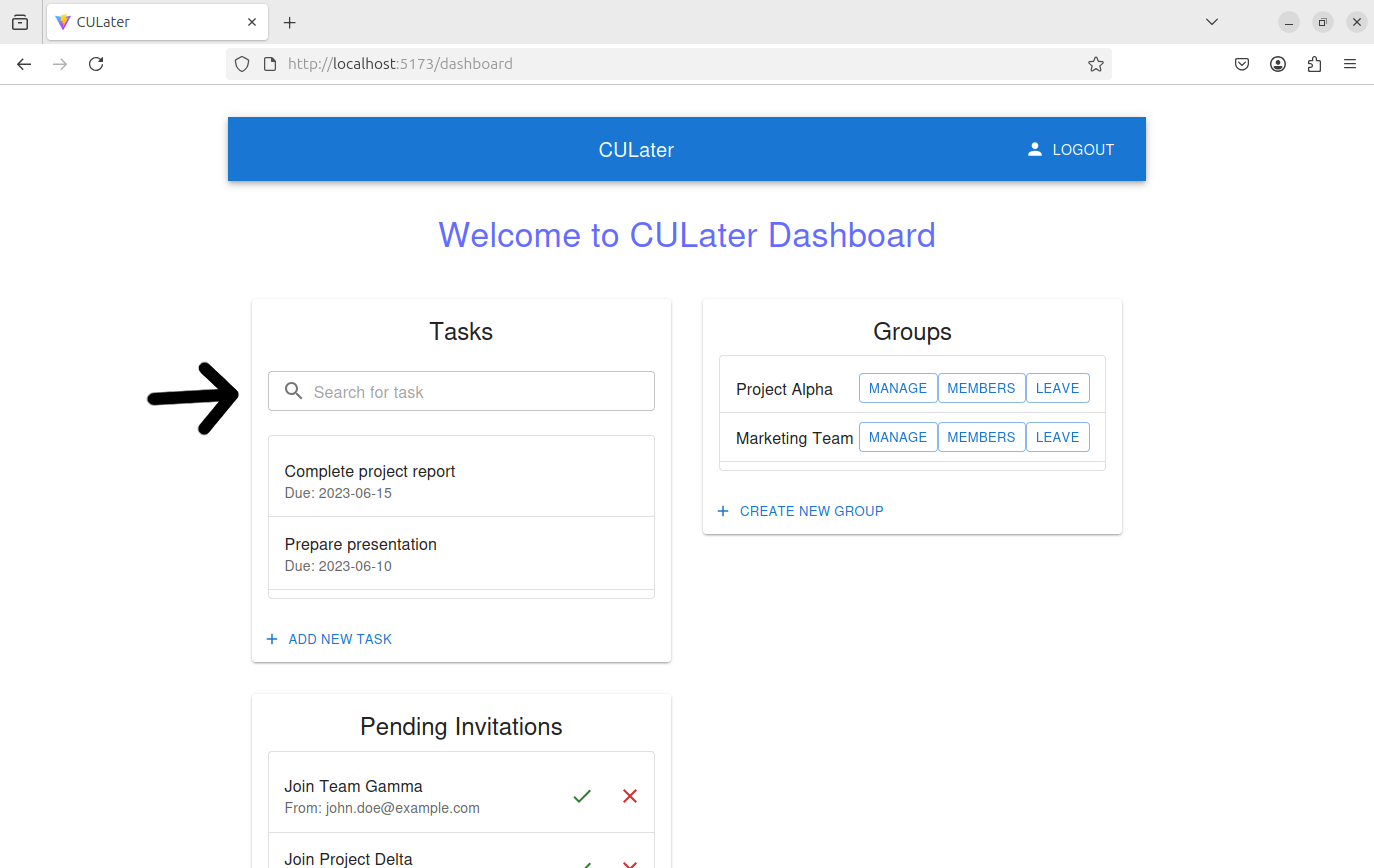
\includegraphics[width=0.8\textwidth]{task_filtering.png}
	\caption{Task filtering}
	\label{fig:my_label}
\end{figure}

\chapter{Group Invitations}

The admins and the contributors of a group can invite other users to the group. For this, the user requests to share the group. Then, they are asked to provide the users they would like to invite and the type of tole they want to give to the invitee. A user can only grant less or the same permissions as themselves. After submitting, the invite is sent. The invitee can view the invite on their dashboard.\\

To accept/decline an invite, simply either click on the tick sign or the cross sign. Once you accept an invitation, you will see your new group among your groups on your dashboard, and you will be able to view the tasks of that group.\\
\begin{figure}[htbp]
        \centering
        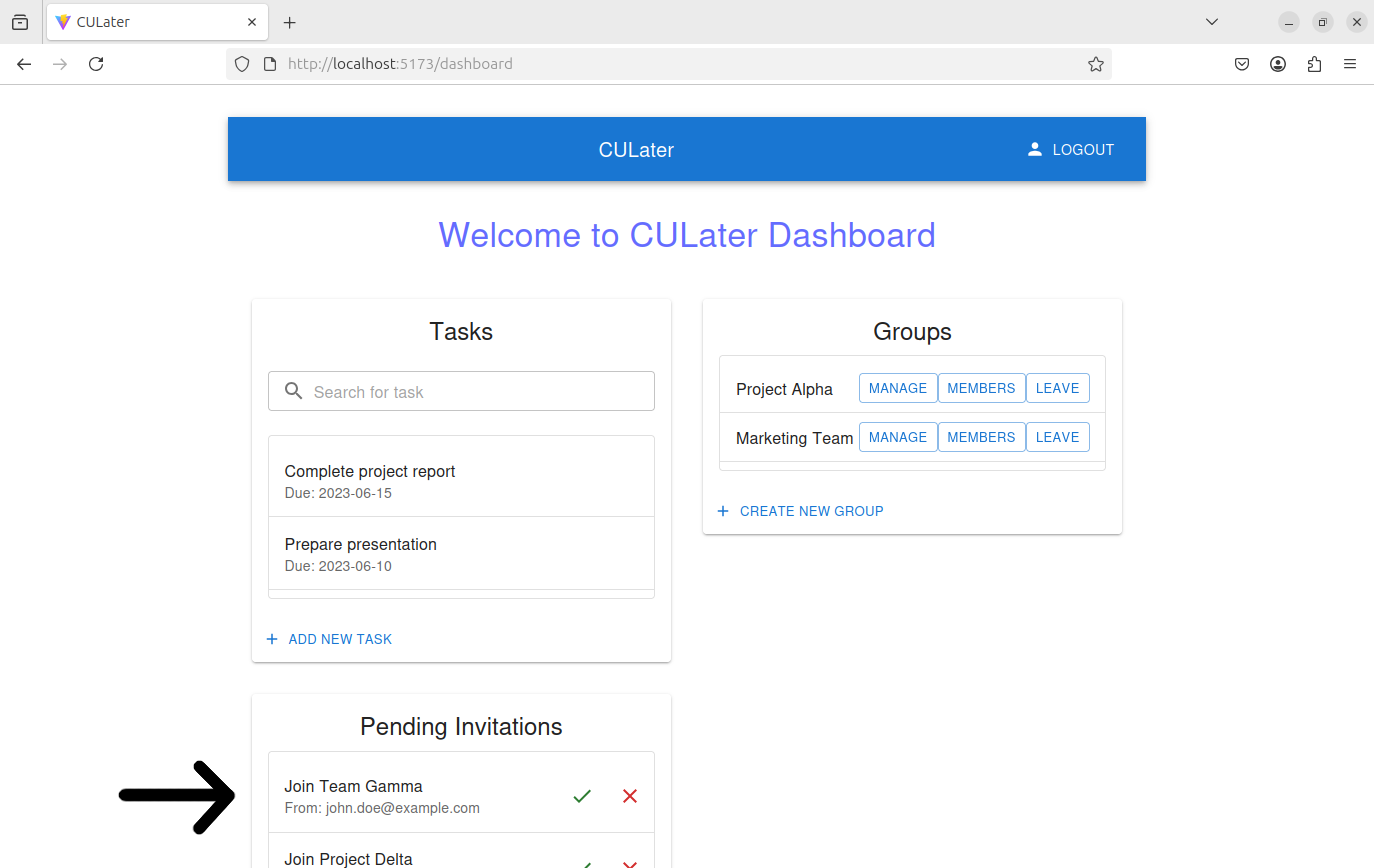
\includegraphics[width=0.8\textwidth]{invitation.png}
	\caption{Viewing/accepting/declining invitations}
	\label{fig:my_label}
\end{figure}

\chapter{Viewing Group Details}

On the "Groups" tab on the dashboard, each group has a "MANAGE" and "MEMBERS" button next to the group name. Users that are members of the group can view the group description by clicking on "MANAGE" and view the members by clicking on "MEMBERS".\\
\begin{figure}[htbp]
        \centering
        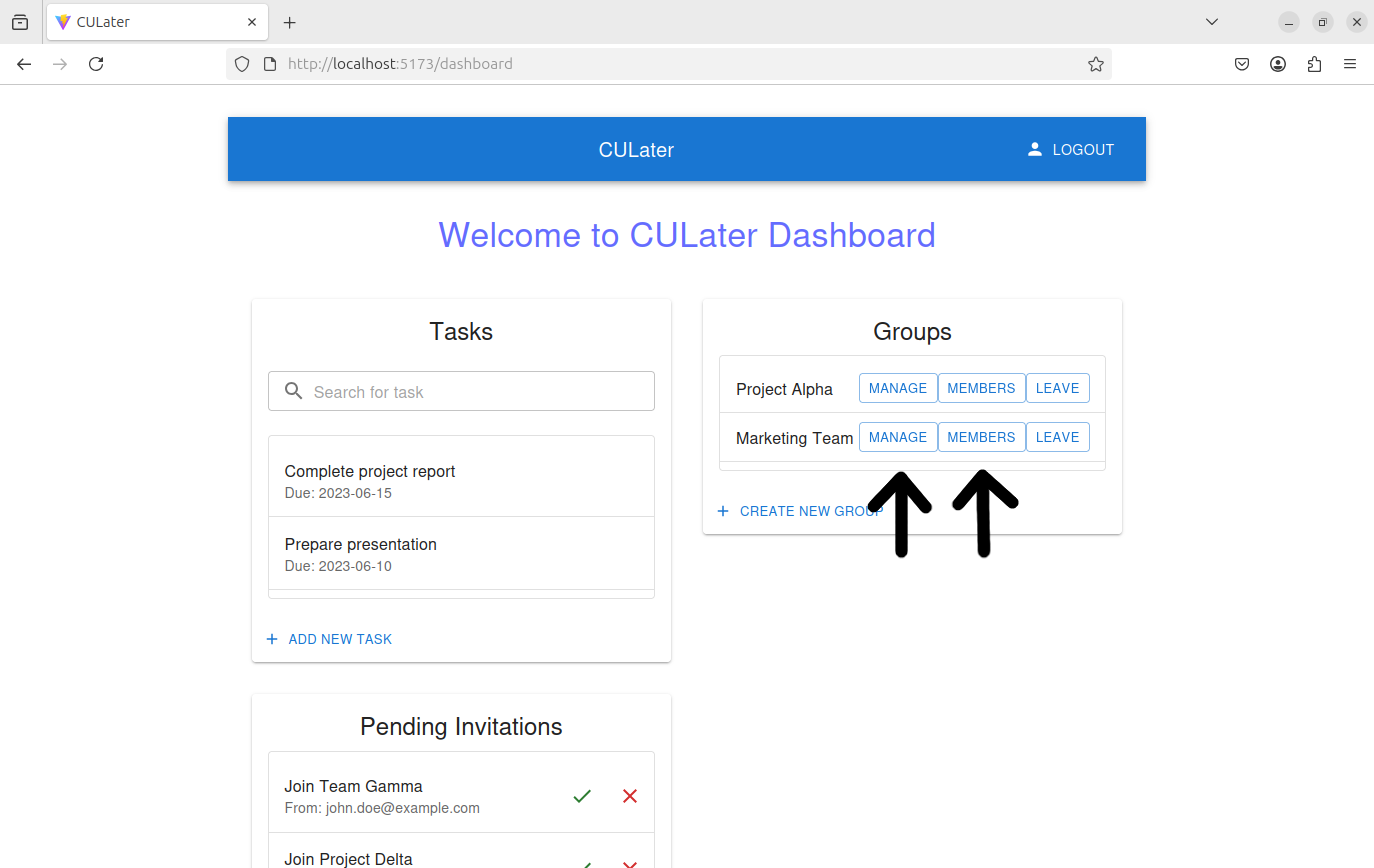
\includegraphics[width=0.8\textwidth]{group_details.png}
	\caption{Group details on dashboard}
	\label{fig:my_label}
\end{figure}
\begin{figure}[htbp]
        \centering
        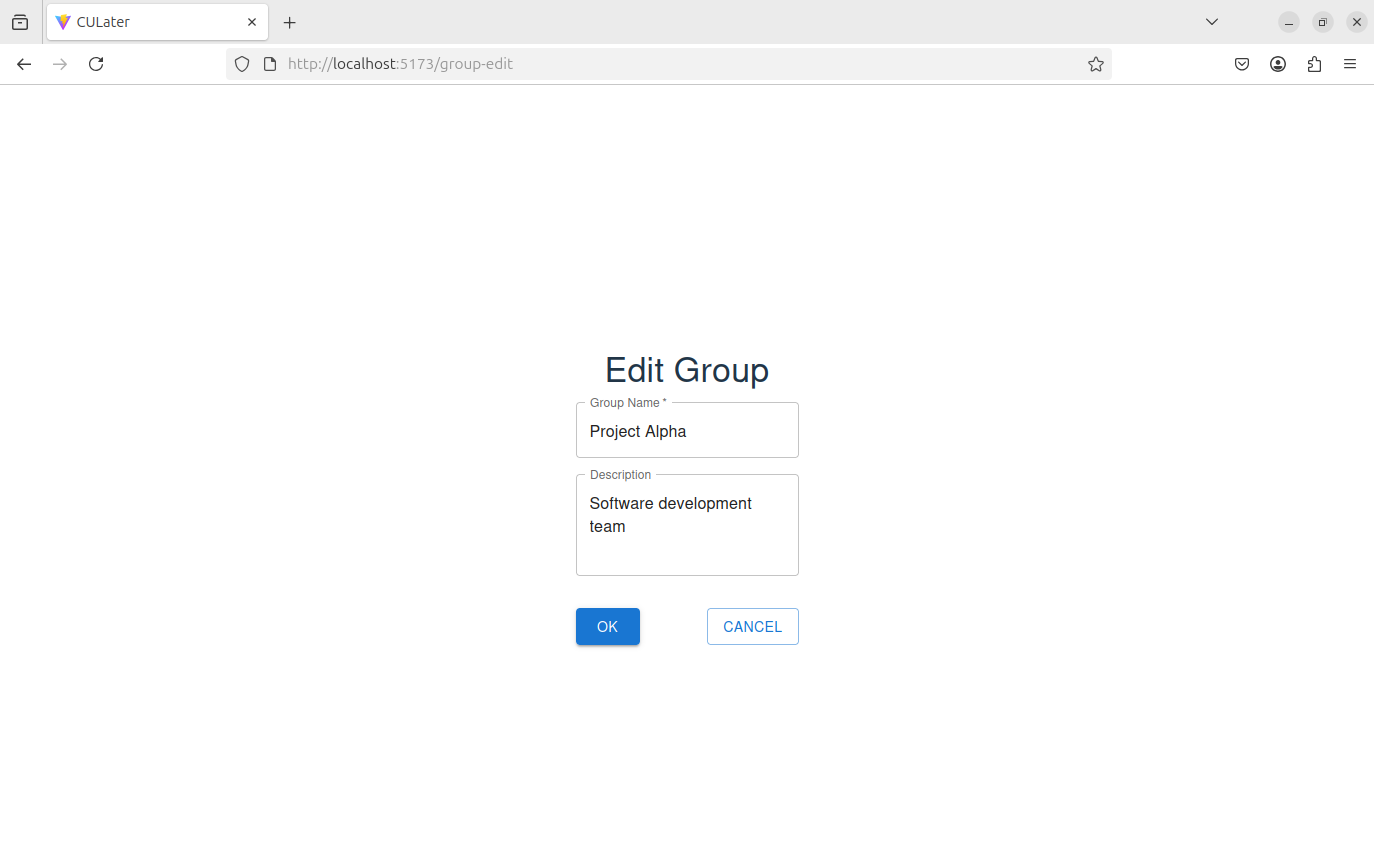
\includegraphics[width=0.8\textwidth]{group_update.png}
	\caption{Viewing group details}
	\label{fig:my_label}
\end{figure}
\begin{figure}[htbp]
        \centering
        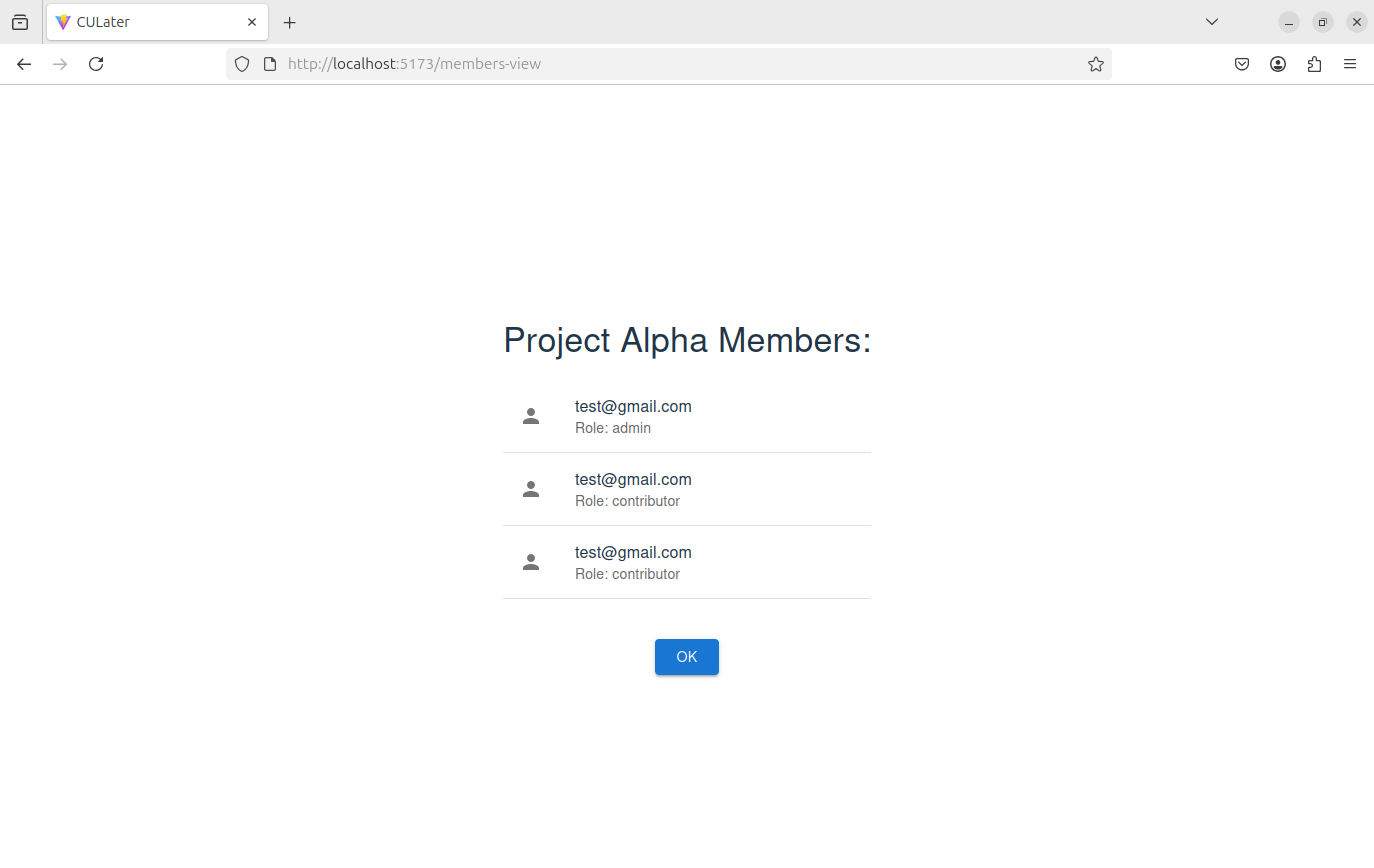
\includegraphics[width=0.8\textwidth]{show_members.png}
	\caption{Viewing group members}
	\label{fig:my_label}
\end{figure}


\chapter{Updating Group Details}

Only Admins of a group can update the group details. If you are the admin of a group, you can update the group details by clicking "MANAGE" next to the group name on your dashboard. Once you are on the group update page, do the necessary changes and submit. If you attempt to change the group details of a group where you are not an admin, an error will be prompted.\\
\begin{figure}[htbp]
        \centering
        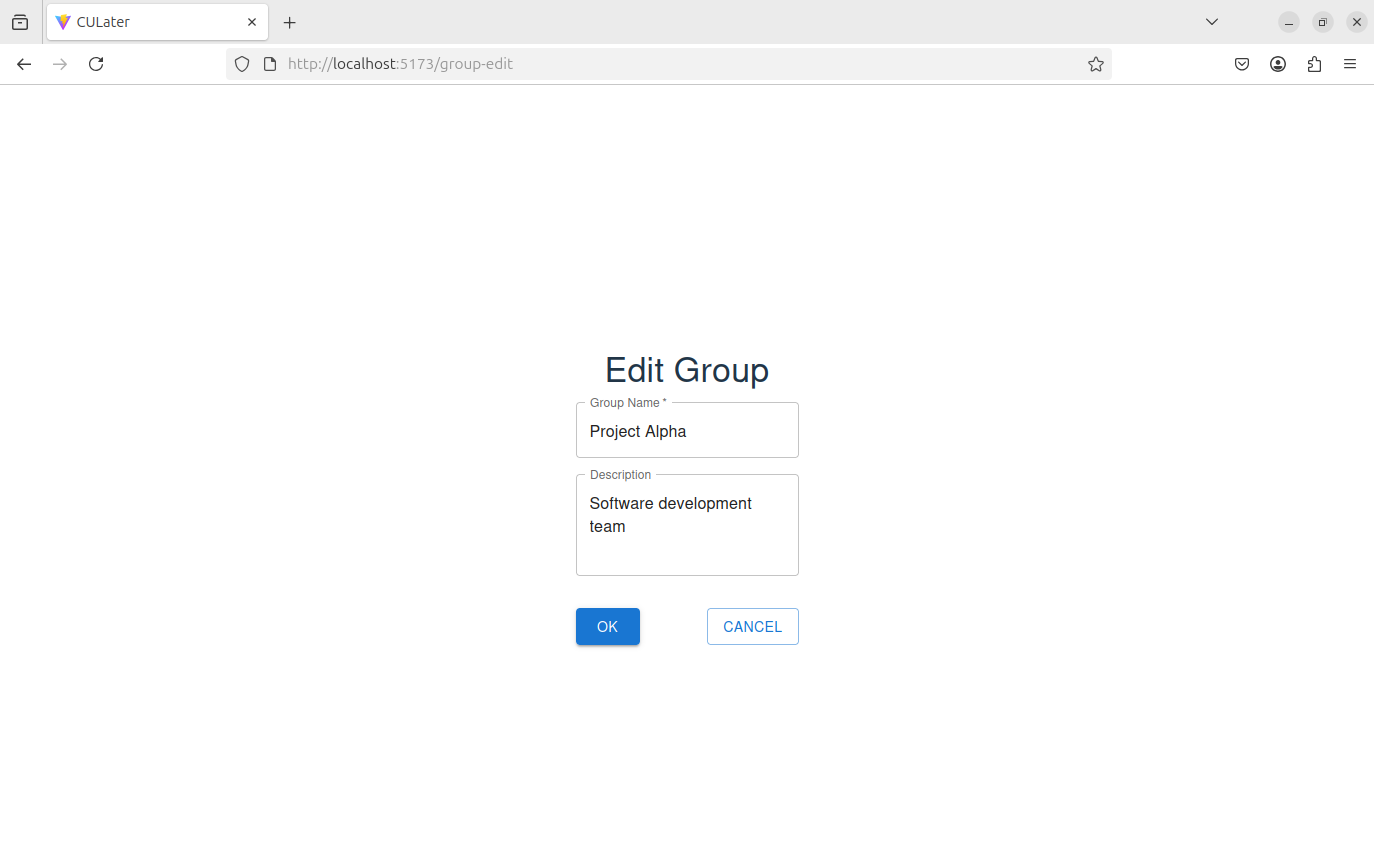
\includegraphics[width=0.8\textwidth]{group_update.png}
	\caption{Updating group details}
	\label{fig:my_label}
\end{figure}

\chapter{Leaving A Group}

To leave a group, simply click on the "LEAVE" box next to the group name on the dashboard. The group will be removed from your dashboard. If you are a group admin, another random user will be assigned the admin of the group once you leave.\\
\begin{figure}[htbp]
        \centering
        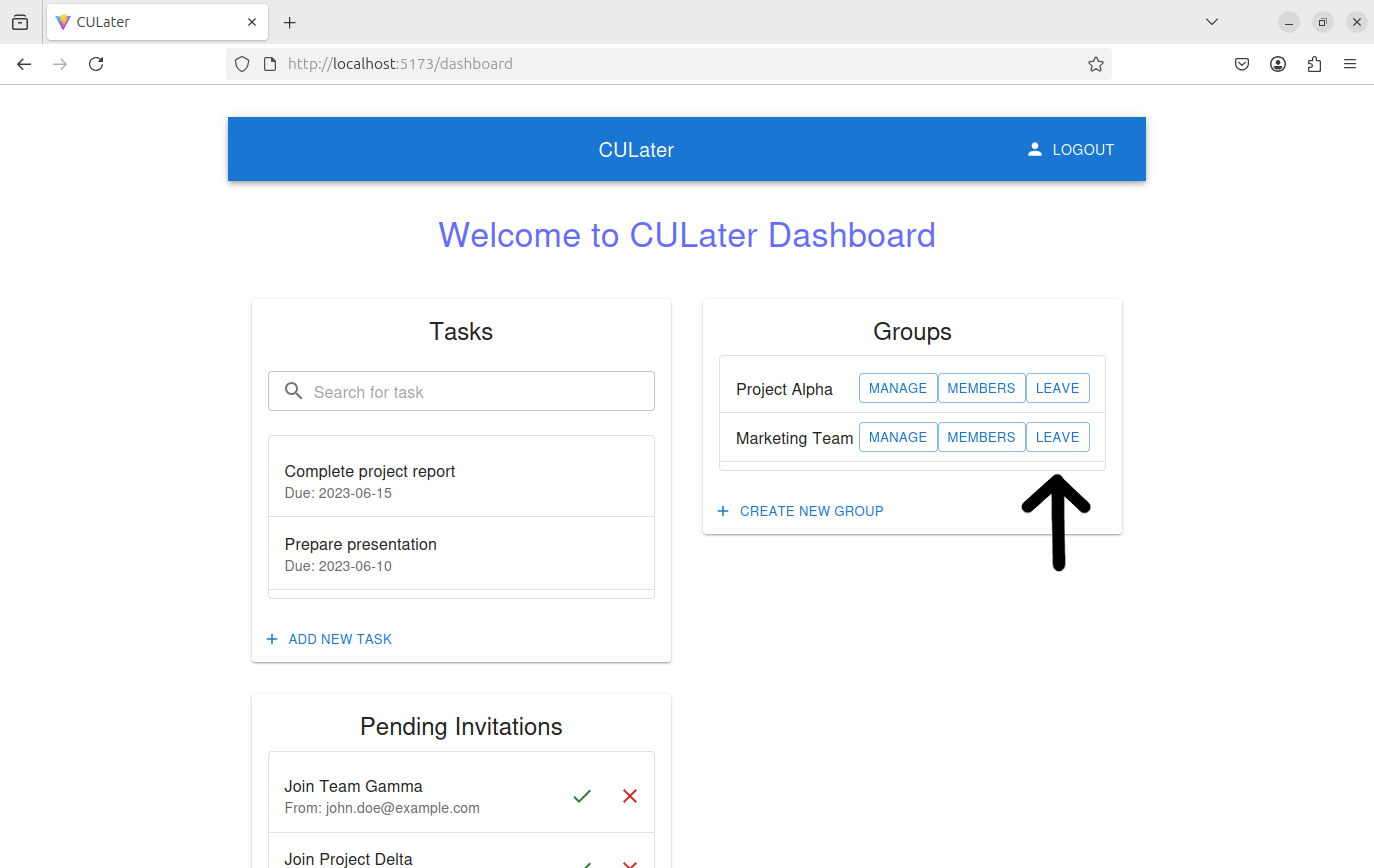
\includegraphics[width=0.8\textwidth]{leave_group.png}
	\caption{Leaving a group}
	\label{fig:my_label}
\end{figure}


\end{document}
